\documentclass{article}

\title{Assigment2 - RNA \& Assembly}
\date{\today}
\author{Weize Xu}

\usepackage{sectsty}
\sectionfont{\fontsize{12}{12}\selectfont}

\usepackage{geometry}
\geometry{
    a4paper,
    total={170mm,257mm},
    left=30mm,
    right=20mm,
    top=20mm,
    }
   
\renewcommand{\baselinestretch}{1.2}

\usepackage[linesnumbered,boxed,lined]{algorithm2e}

\usepackage{graphicx}
\usepackage{subcaption}

\usepackage{hyperref}
\hypersetup{
    colorlinks=true,
    linkcolor=blue,
    filecolor=magenta,      
    urlcolor=cyan,
}

\usepackage{listings}


\begin{document}

\maketitle

\section{Can you give the pseudocode for the Nussinov folding algorithm? Also, please
         describe the algorithm to recover the secondary structure.}

\large{\textbf{Answer:}}

Nussinov folding algorithm is a kind of Dynamic Programming algorithm, 
which goal is to maximize the folding pairs. Pseudocode see Algorithm \ref{alg:Nussinov}. \\


\section{Consider the set of reads \{ACCTCC, TCCGCC, CCGCCA\}. For k=2 or 3,
         can you build a de Brujin graph $H_k$ ? Can you get the Eulerian path from $H_k$ ? Is
         the Eulerian path unique?}

\large{\textbf{Answer:}}

I wrote a little script for building and drawing the de Brujin graph. 
see \url{https://github.com/Nanguage/Course-Algorithms-in-Bioinformatics/blob/master/L04/debrujin.py}.
Figure \ref{fig:q2} show the de Burjin graph when $k=2$ and $k=3$.

\begin{figure}[h]
    \begin{subfigure}[h]{0.35\linewidth}
        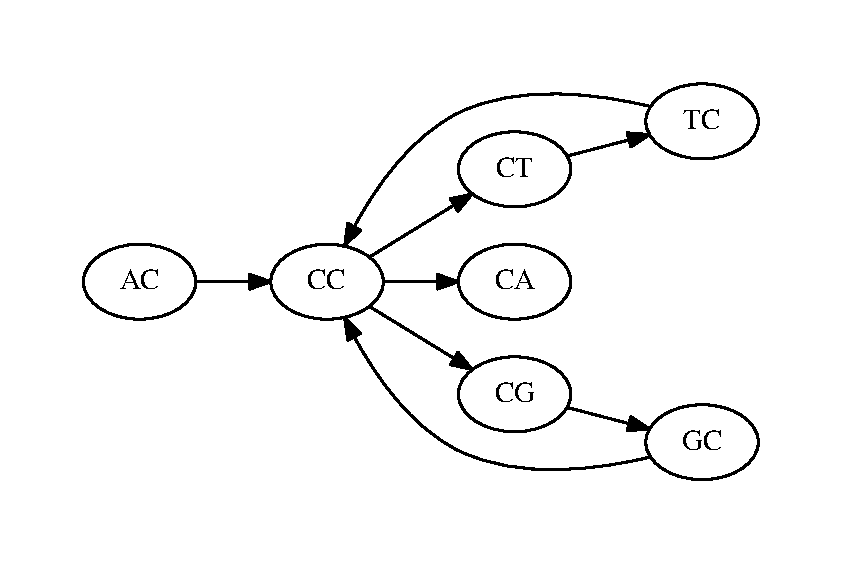
\includegraphics[width=\linewidth]{./img/q2-k2.pdf}
        \caption{$k=2$}
    \end{subfigure}
    \begin{subfigure}[h]{0.65\linewidth}
        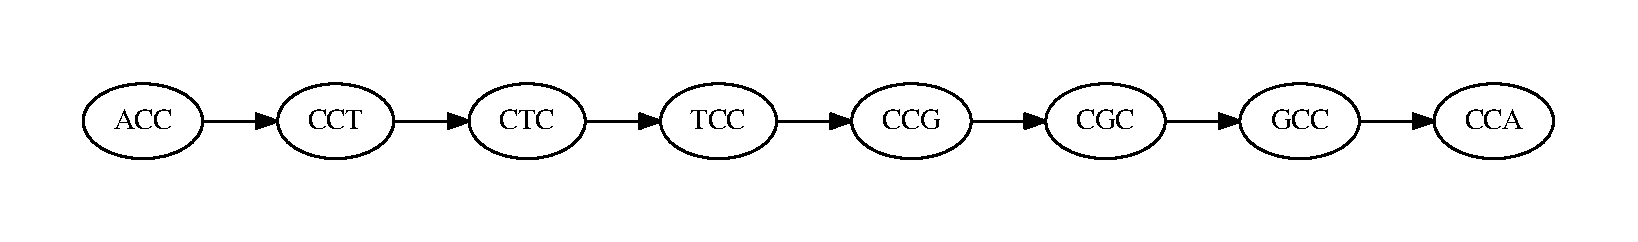
\includegraphics[width=\linewidth]{./img/q2-k3.pdf}
        \caption[b]{$k=3$}
    \end{subfigure}
    \caption{de Burjin graph $H_k$ when $k=2$ and $k=3$}
    \label{fig:q2}
\end{figure}

Obvirously, when $k=3$ there are just one unique euler path.
But when $k=2$, there are two euler paths:

\begin{quote}
    $AC \rightarrow CC \rightarrow CT \rightarrow TC \rightarrow CC \rightarrow CG \rightarrow GC \rightarrow CC \rightarrow CA$ \\
    $AC \rightarrow CC \rightarrow CG \rightarrow GC \rightarrow CC \rightarrow CT \rightarrow TC \rightarrow CC \rightarrow CA$ 
\end{quote}

\section{Suppose T = \{ACT, CAC, CTG, CTT, TCA, TTC\} and R = CTGCACT. Can
you compute the minimum edit distance between R and a T-string? Please
illustrate the steps.}

\large{\textbf{Answer:}}

I implemented the dynamic programming algorithm 
for solving the Spectral alignment problem(SAP).
Source code see \\
\url{https://github.com/Nanguage/Course-Algorithms-in-Bioinformatics/blob/master/L04/sap.py} \\
According to my program's computation, the minimum edit distance is 1.


\begin{algorithm}[]

    \SetKwInOut{Input}{input}\SetKwInOut{Output}{output}
    \SetKwFunction{Initialize}{InitializeMatrix}
    \SetKwFunction{Matrix}{Matrix}
    \SetKwFunction{Max}{Max}
    \SetKwFunction{Traceback}{Traceback}

    \SetKwProg{Fn}{procedure}{}{end}

    \Input{An RNA sequence $S[1..n]$}
    \Output{A set of pairs $P$}
    \BlankLine

    $V \leftarrow$ \Matrix{n, n}\\
    \Initialize{$V$, $n$}

    \For {$m \leftarrow 1$ \KwTo $(n-1)$} {
        \For{$i \leftarrow 1$ \KwTo $(n-m)$} {
            $j \leftarrow i + m$ \\
            $v_0 \leftarrow$ $V[i,j] + \delta$(S[i], S[j]) \\
            $v_1 \leftarrow 0$ \\
            \For{$k \leftarrow i$ \KwTo $j$} {
                $v \leftarrow V[i, k] + V[k+1, j]$ \\
                \If{$v > v_1$} {
                    $v_1 \leftarrow v$
                }
            }
            $V[i, j] \leftarrow$ \Max{$v_0$, $v_1$}
        }
    }
    $P \leftarrow \{\}$ \\
    \Traceback{$P$, V, $1$, $n$} \\
    \Return $P$

    \BlankLine

    \Fn{\Initialize{Mat, n}} {
        \For{$i \leftarrow$ 1 \KwTo $n$} {
            $Mat[i, i] \leftarrow$ 0 \\
            \If {$i \neq n$} {
                $Mat[i+1, i] \leftarrow$ 0
            }
        }
    }

    \BlankLine

    \Fn{\Traceback{Pairs, V, i, j}} {
        \uIf{$j \leq i$} {
            \Return
        }
        \uElseIf{$V[i,j] = V[i,j-1]$} {
            \Traceback{$Pairs$, $V$, $i$, $j-1$} \\
            \Return
        }
        \Else {
            \For{$k \leftarrow i$ \KwTo $j$} {
                \If{$\delta(S[k], S[j]) \neq 0$} {
                    $Pairs \cup (k, j)$ \\
                    \Traceback{$Pairs$, $V$, $i$, $k-1$} \\
                    \Traceback{$Pairs$, $V$, $k+1$, $j-1$} \\
                    \Return
                }
            }
        }
        
    }

    \caption{Nussinov folding}
    \label{alg:Nussinov}

\end{algorithm}

\end{document}
